\documentclass{beamer}
\mode<presentation>
%%Import
%\usepackage[ngerman]{babel}
\usepackage[utf8]{inputenc}
\usepackage{graphicx}
\usepackage{listings}
\usepackage{hyperref}

%%Layout
\usetheme{Singapore}
\usecolortheme[cmyk={1,0.7,0,0}]{structure}
%\setbeamercovered{transparent}
\beamertemplatenavigationsymbolsempty
\setbeamertemplate{footline}[frame number]

%%Meta-Daten
\title{Endterm Presentation - Safety Car}
\subtitle{HW/SW-Co-design with (LEGO)Cars}
\author{Florian, Chris and Lukas}
\institute[TUM]{Technische Universität München}
\date{3rd February 2014}
\logo{
\includegraphics[scale=0.5]{LogoFMI.png}}

\begin{document}

\begin{frame}
	\titlepage
\end{frame}

\begin{frame}
	\frametitle{Content}
	\tableofcontents
\end{frame}

\section{HW Setup}

\subsection{Car-Design}

\begin{frame}
	\frametitle{Hardware Overview}
	Key-Components:
	\begin{itemize}
		\item \textit{wooden chassis}, aprox. 40 cm x 35 cm
		
		\item \textit{12.6 V battery} with continuous 90 A ($\Rightarrow$ 1134 W!)\\
		Central power-management\\
		(generating 5 V for FPGAs / Linux-PC and 9 V for Ethernet-Switch)	
	
		\item \textit{4 CMWUnits} (ControlMotorWheel-Unit) see next slide...
		
		\item \textit{Linux-PC} which controls every CMWUnit and sensor
		
		\item \textit{Ultrasound-Sensors}
	\end{itemize}
\end{frame}

\begin{frame}
	\frametitle{Car Design - Overview}
	\begin{figure}
	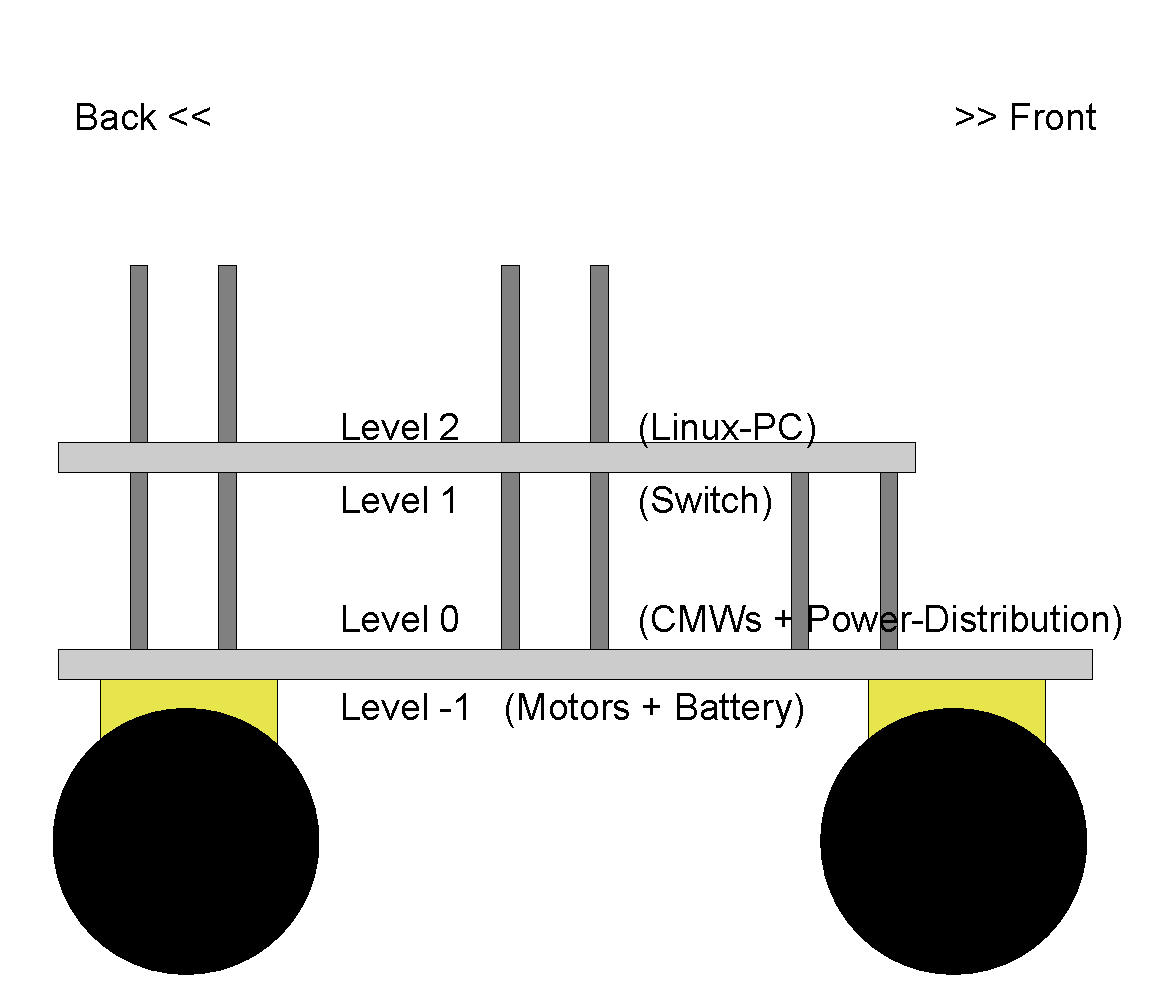
\includegraphics[scale=0.4]{figures/overview.pdf}
	\caption{The car is divided into four levels. Each level has a different motto.}
	\end{figure}
\end{frame}

\begin{frame}
	\frametitle{Level -1}
	\begin{figure}
	\includegraphics[scale=0.7]{figures/level-1_b.jpg}
	\caption{The lowest level contains the four motors and the battery.}
	\end{figure}
	
\end{frame}

\begin{frame}
	\frametitle{Level 0}
	\begin{figure}
	\includegraphics[scale=0.7]{figures/level0_b.jpg}
	\caption{Level 0 contains the CMW-Units and the Voltage-Distribution}
	\end{figure}
\end{frame}

\begin{frame}
	\frametitle{CMWUnit - Control-Motor-Wheel-Unit}
	Each Control-Motor-Wheel(CMW)-Unit consists of:
	\begin{itemize}	
		\item One \textit{Ethernet-UART} connected to the central FPGA
	
		\item One \textit{DE0Nano-Boards} (FPGA)
		
		\item One \textit{H-Bridge}	(dual-channel but we only use one channel)
	
		\item One \textit{Pololu Motor} (max. power: 60 W @ 12 V, 5 A).\\
		Problem: Many components can not take over 2 A! 
		
		\item One \textit{Soft-Wheel} (diameter: aprox. 12 cm)\\
		Problem: Each Soft-Wheel can take max. 3 kg 
	\end{itemize}
\end{frame}

\begin{frame}
	\frametitle{CMWUnit - Control-Motor-Wheel-Unit}
	\begin{figure}
	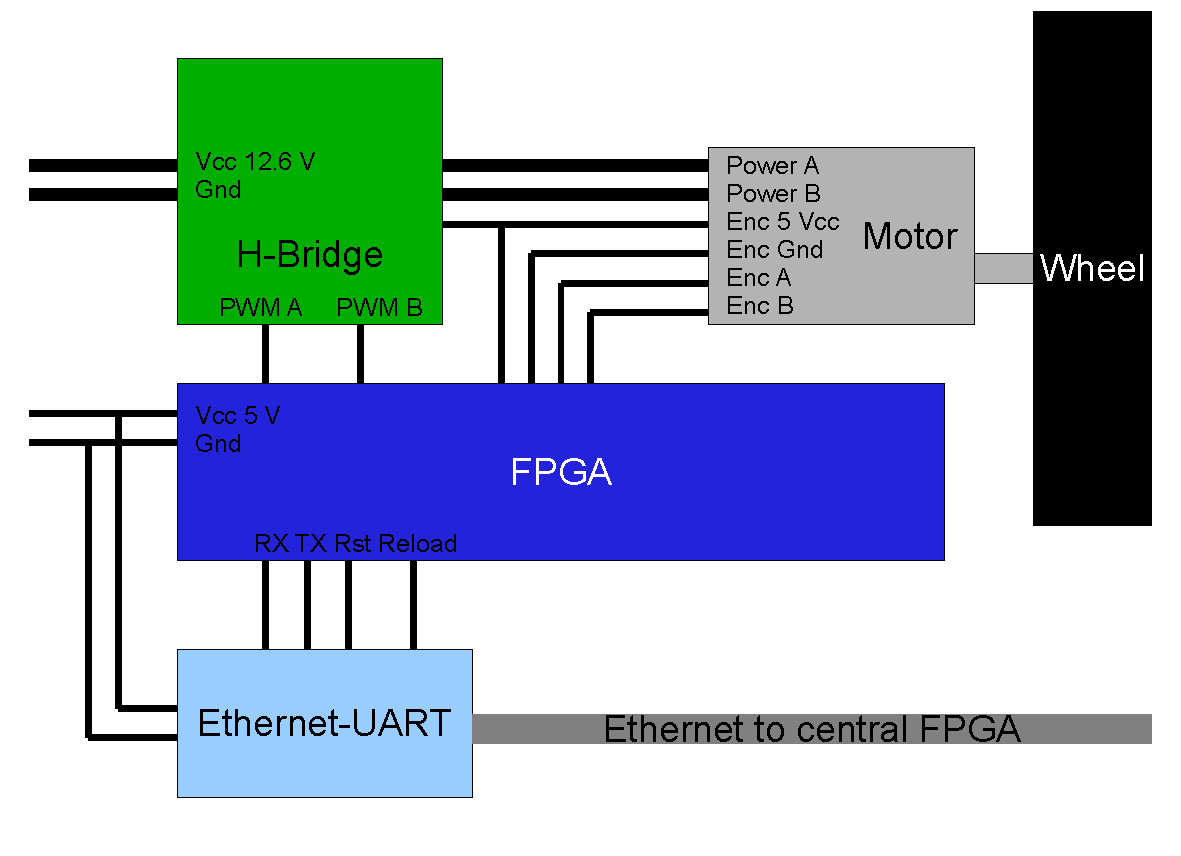
\includegraphics[scale=0.5]{figures/cmwunit.pdf}
	\caption{Interconnections in the Control-Motor-Wheel-Unit}
	\end{figure}
\end{frame}

\begin{frame}
	\frametitle{Level 1}
	\begin{figure}
	\includegraphics[scale=0.7]{figures/level1_b.jpg}
	\caption{Level 1 contains the Ethernet-Switch}
	\end{figure}
\end{frame}

\begin{frame}
	\frametitle{Level 2}
	\begin{figure}
	\includegraphics[scale=0.7]{figures/level2_b.jpg}
	\caption{Level 2 contains the (big) Sabre-light i.mx6 (Linux-PC)}
	\end{figure}
\end{frame}

\section{The (great) assembling}

\begin{frame}
	\frametitle{The (great) assembling}
	\begin{itemize}
		\item First issues: Wood or aluminium? Which size?\\ \vspace{1em}
		$\Rightarrow$ Not enough proper aluminium, so take wood!\\
		$\Rightarrow$ We resized the plank three times...\\
		\item Building the first version of power-management.
		\item Then see following process...
	\end{itemize}
\end{frame}

\begin{frame}[fragile]
	\frametitle{The (great) assembling}
	\begin{lstlisting}[language=java, numbers=left, xleftmargin=.03\textwidth]
		while(true){
		    WaitForComponents();
		    GetNewComponents(); 
		                 // Yay!
		    RealiseThatNewComponentsSuitNotForWorkflow();
		                 // :-(
		    ChangeEverythingToImplementNewComponents();
		    SolderANewPowerDistribution(); 
		                 // Burn fingers ;)
		}
		
	\end{lstlisting}
\end{frame}



\section{SW Architecture 1}

\subsection{Our Aims}
\begin{frame}
	\frametitle{Our Aims}
	We want to reach these architectural aims:
	\begin{enumerate}
		\item hierarchical and distributed system\\
		(e.g. separated Motor-Control)
		\item self-maintaining car \\
		(PID calibration, no hardcoded constants, ...)
		\item simple programming of the master-controller (Linux-PC)
	\end{enumerate}
\end{frame}

\subsection{CMW-Unit}

\begin{frame}
	\frametitle{CMW-Unit SW design}
	Processing Unit: \textsl{Nios II} embedded core.\\ \vspace{1em}
	
	Main tasks:
	\begin{enumerate}
		\item Controlling the motor-speed (PI-Controller)
		\item Communicate with Central-Linux-PC
		\item Polling the sensors
	\end{enumerate}
	
	Doing this tasks in a \textbf{hard timed cycle} (as for a real-time system).
\end{frame}

\begin{frame}
	\frametitle{CMW-Unit task cycle}
	Start sequence:\\
	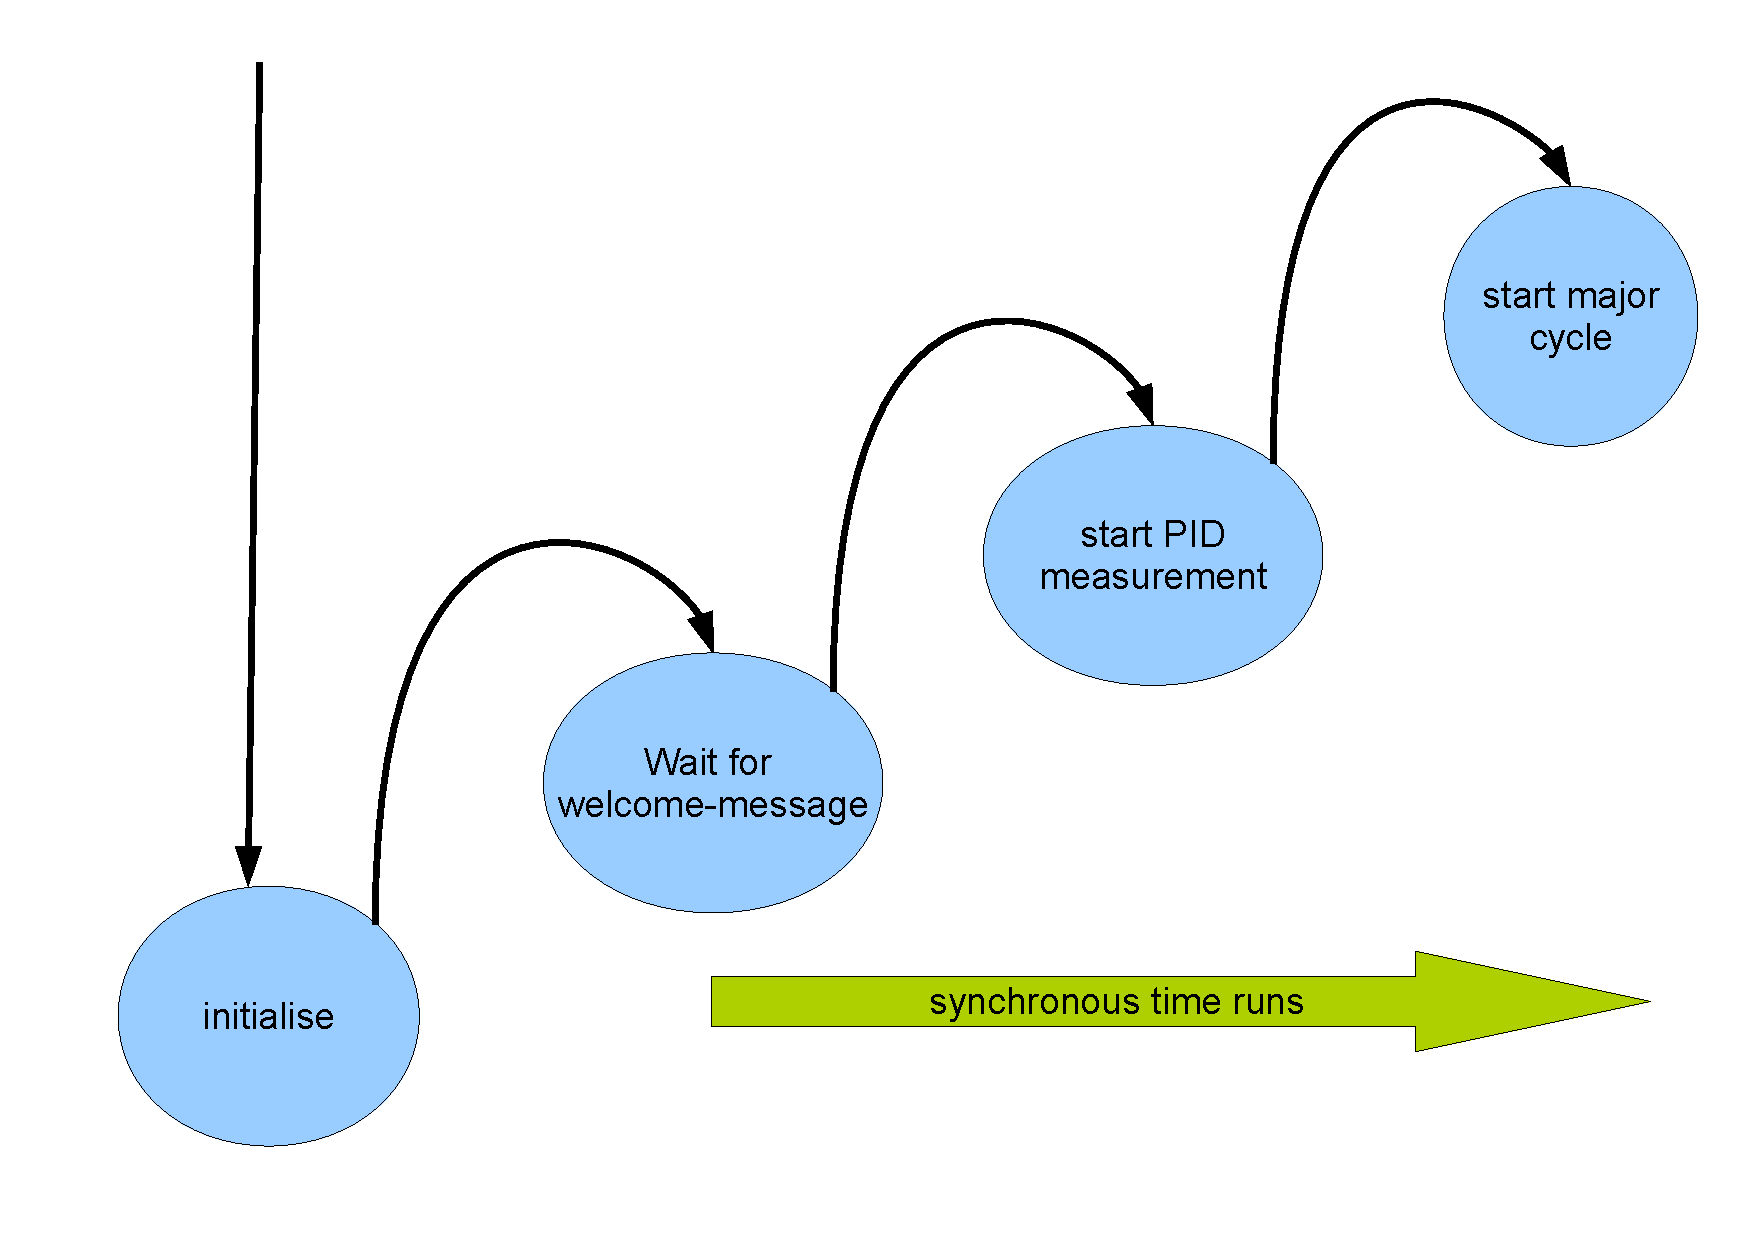
\includegraphics[scale=0.35]{figures/start.pdf}
\end{frame}

\begin{frame}
	\frametitle{CMW-Unit task cycle}
	Major cycle:\\
	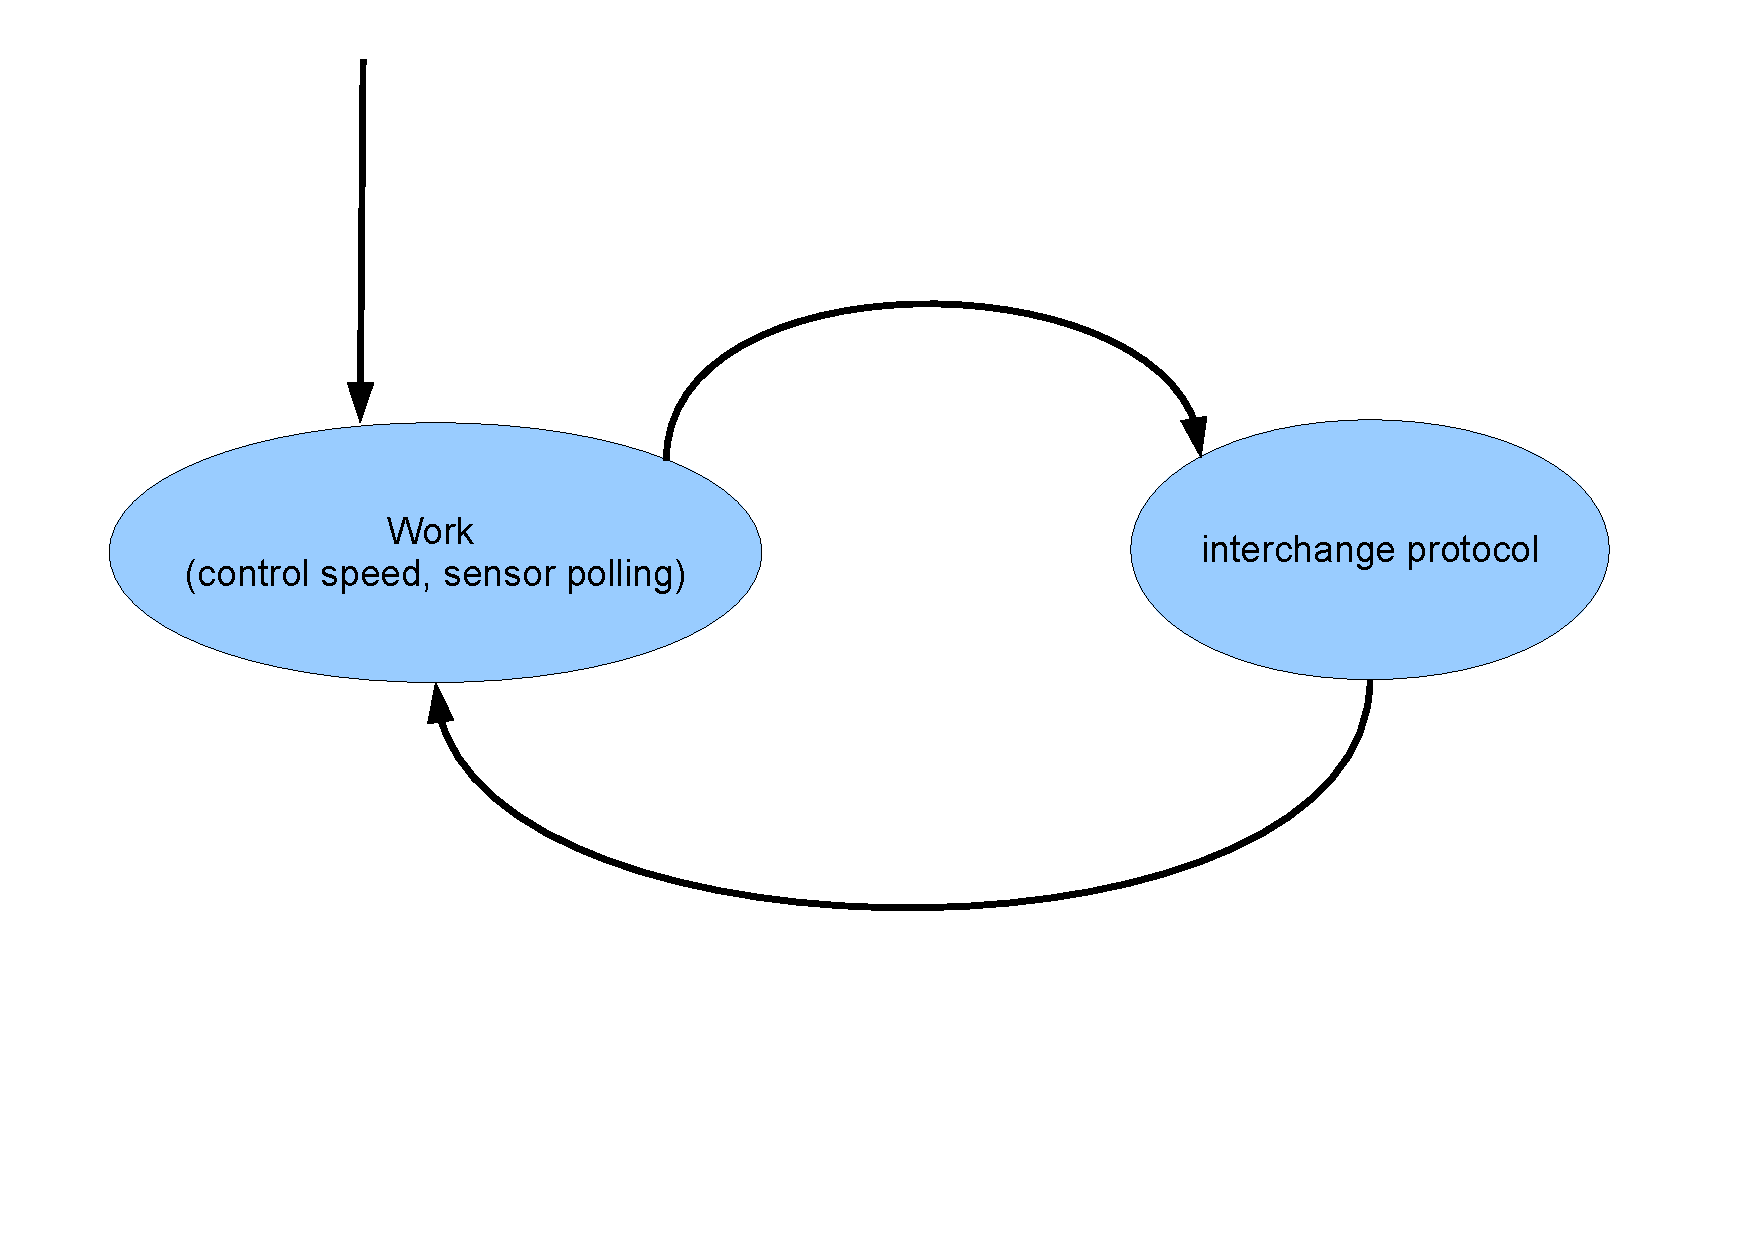
\includegraphics[scale=0.35]{figures/majorcycle.pdf}
\end{frame}

\begin{frame}
	\frametitle{CMW-Unit task cycle}
	Minor cycle:\\
	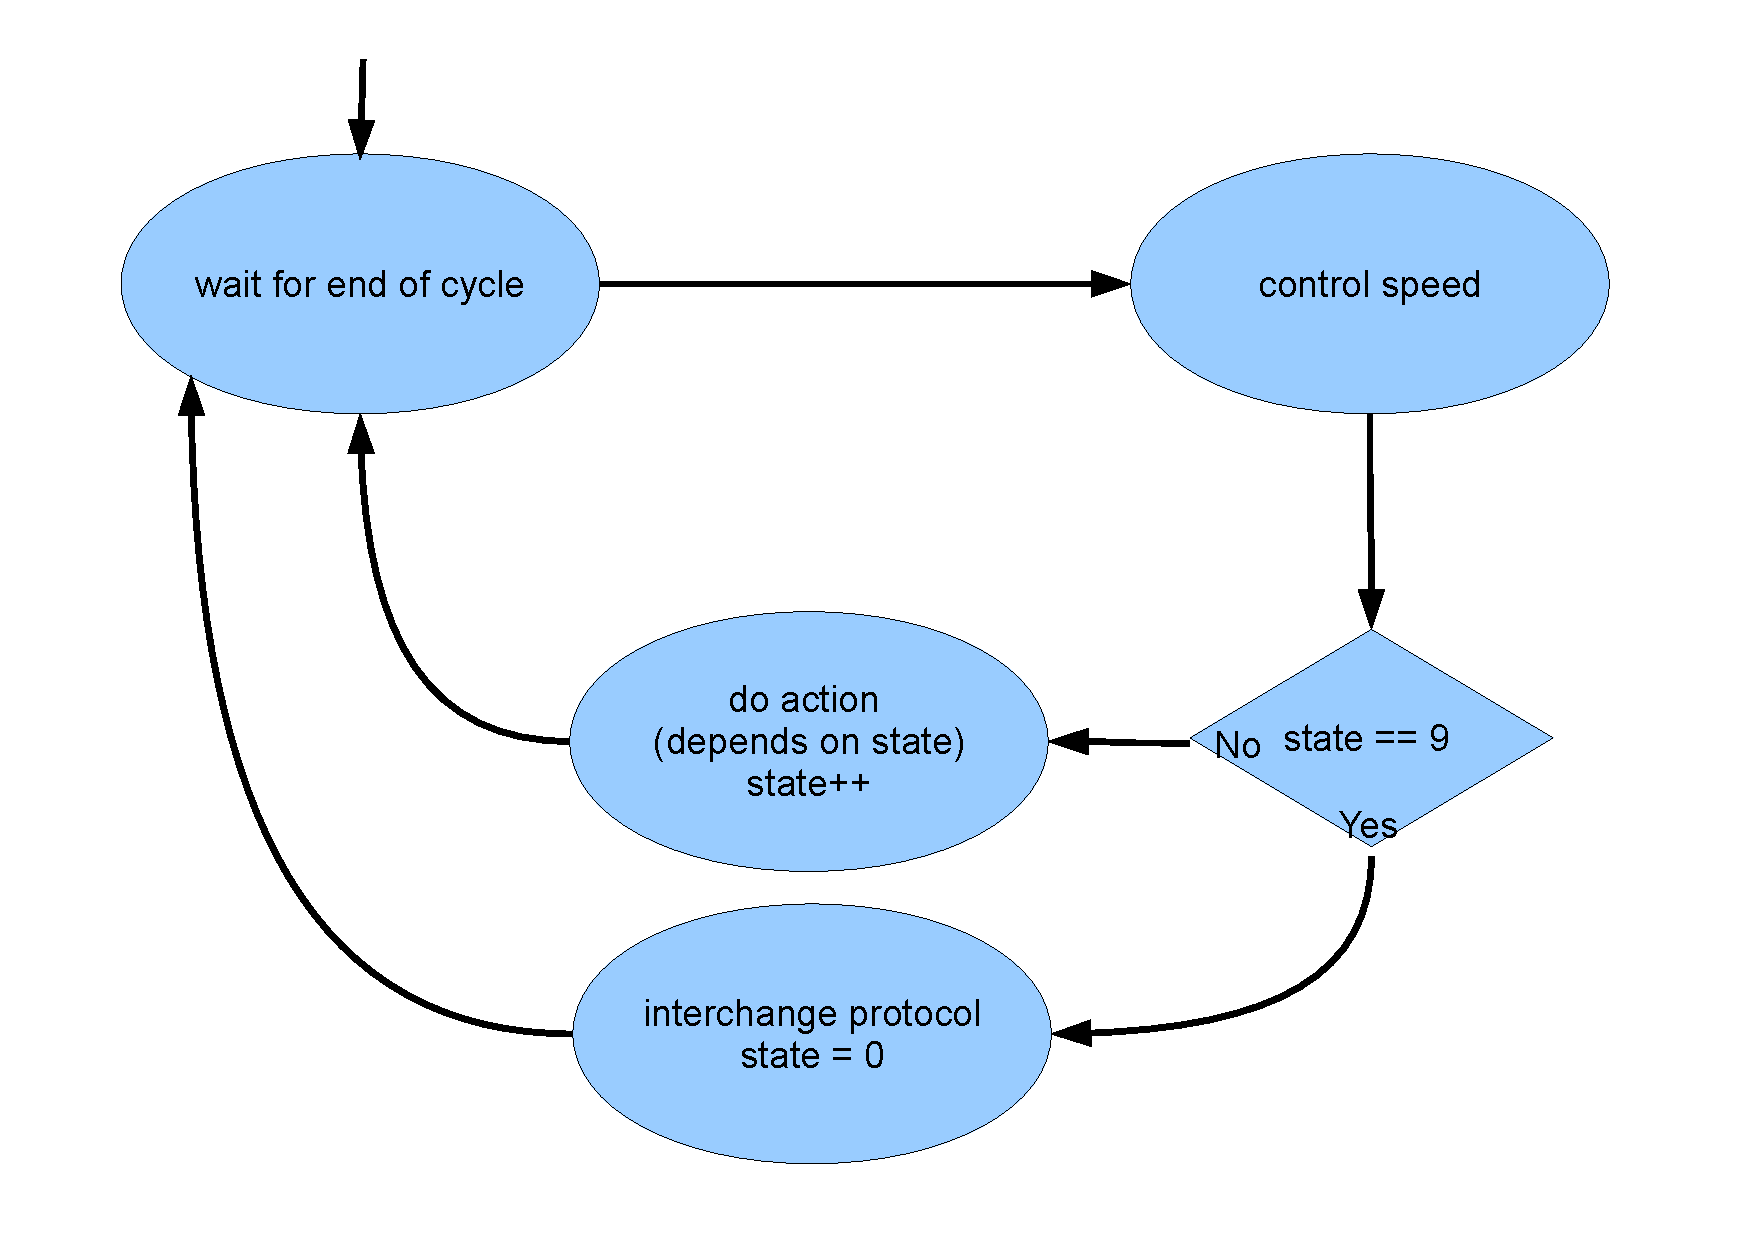
\includegraphics[scale=0.35]{figures/cycle.pdf}
\end{frame}


\subsection{Networking}

\begin{frame}
	\frametitle{Networking Protocol}
	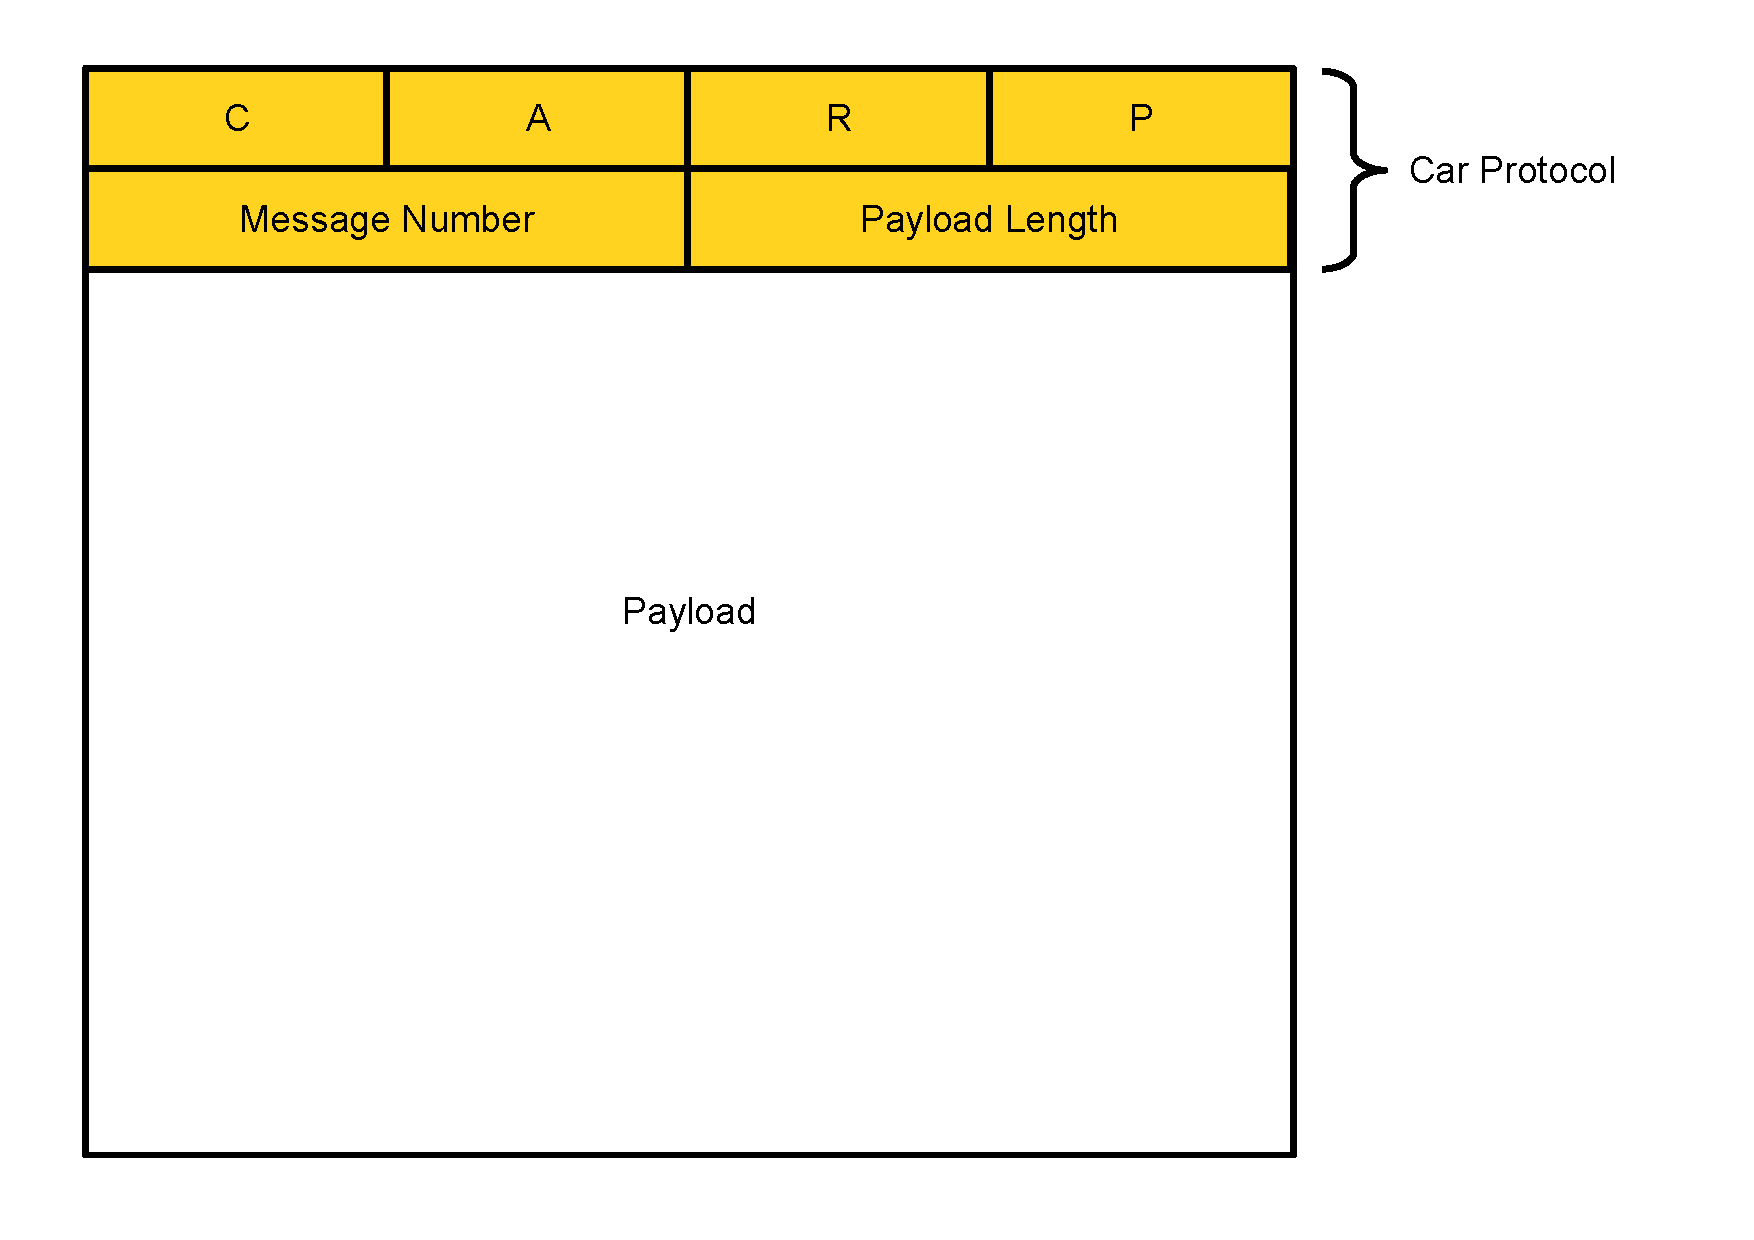
\includegraphics[scale=0.35]{figures/prot0.pdf}
\end{frame}

\begin{frame}
	\frametitle{Networking Protocol}
	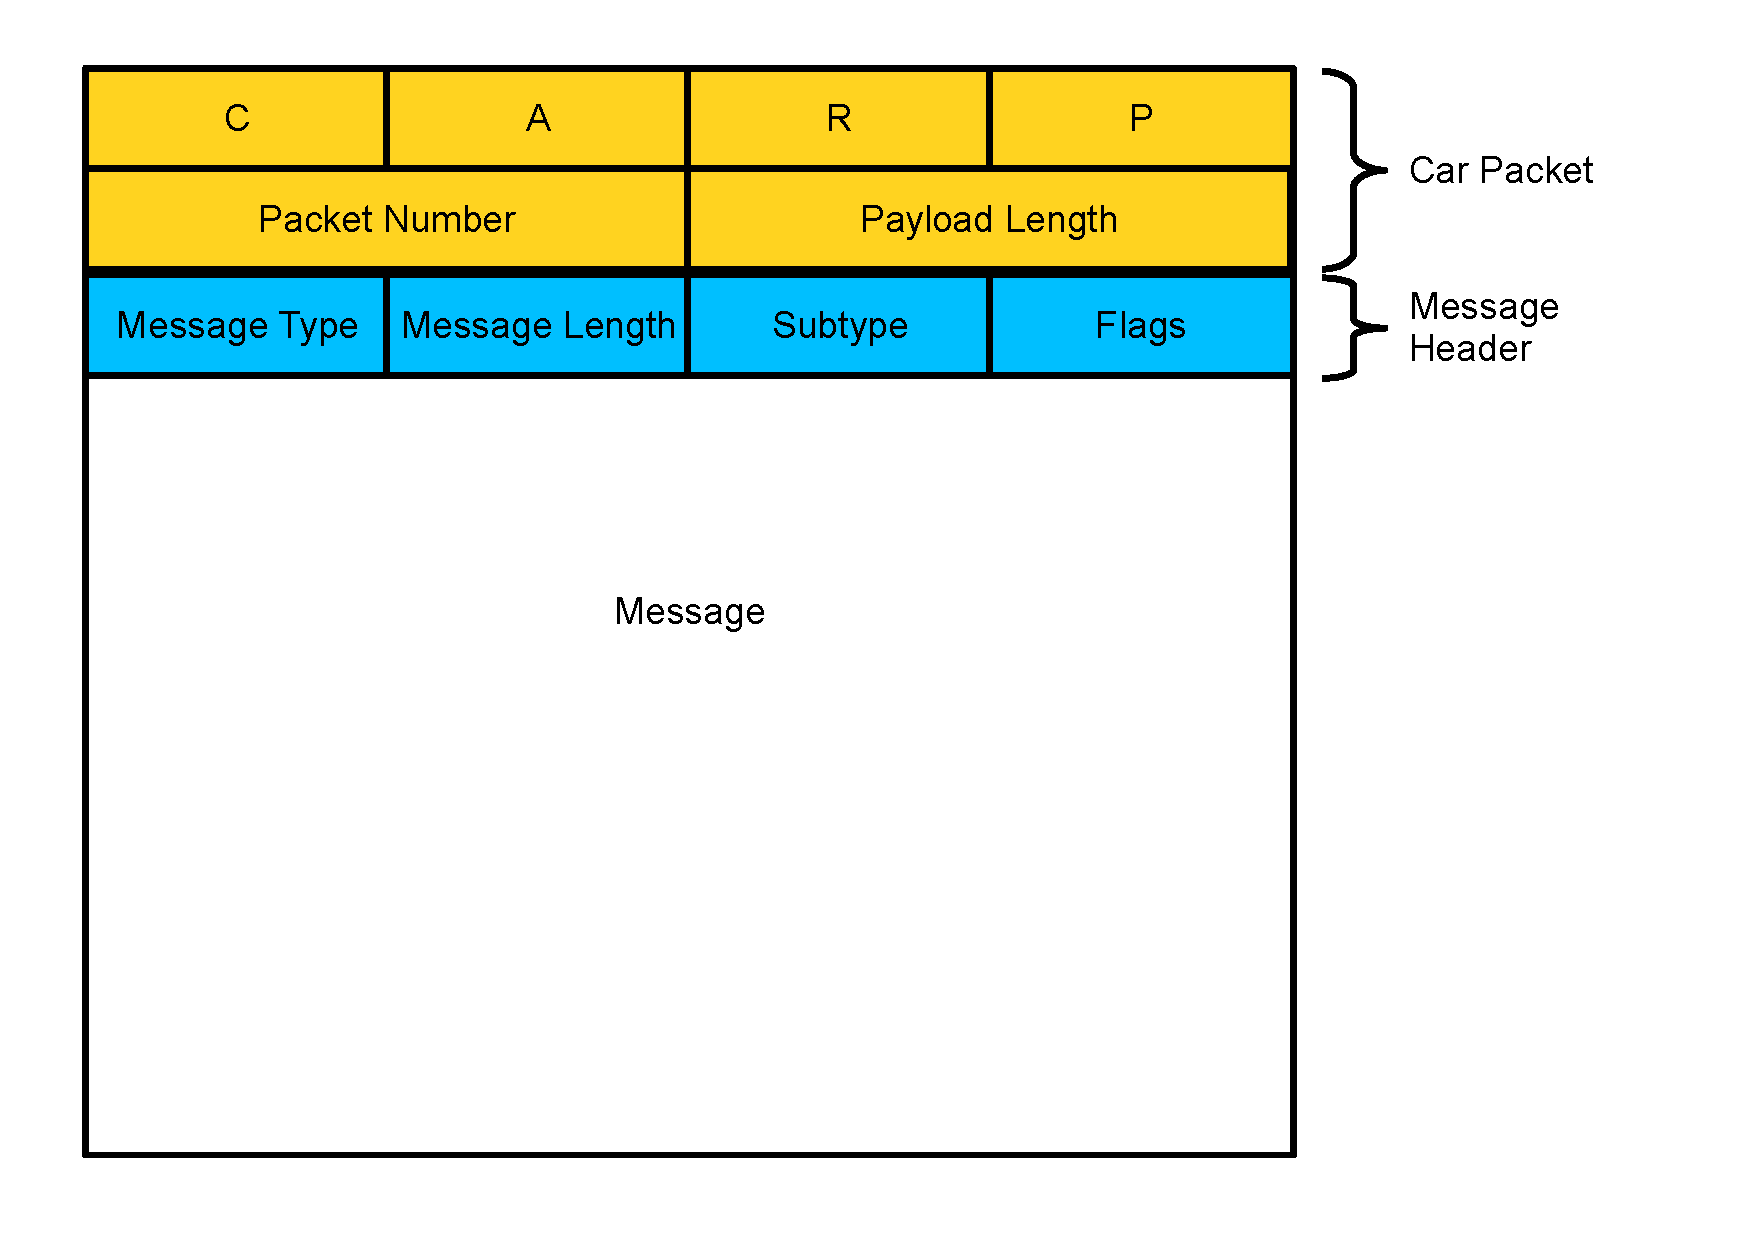
\includegraphics[scale=0.35]{figures/prot1.pdf}
\end{frame}

\begin{frame}
	\frametitle{Networking Protocol}
	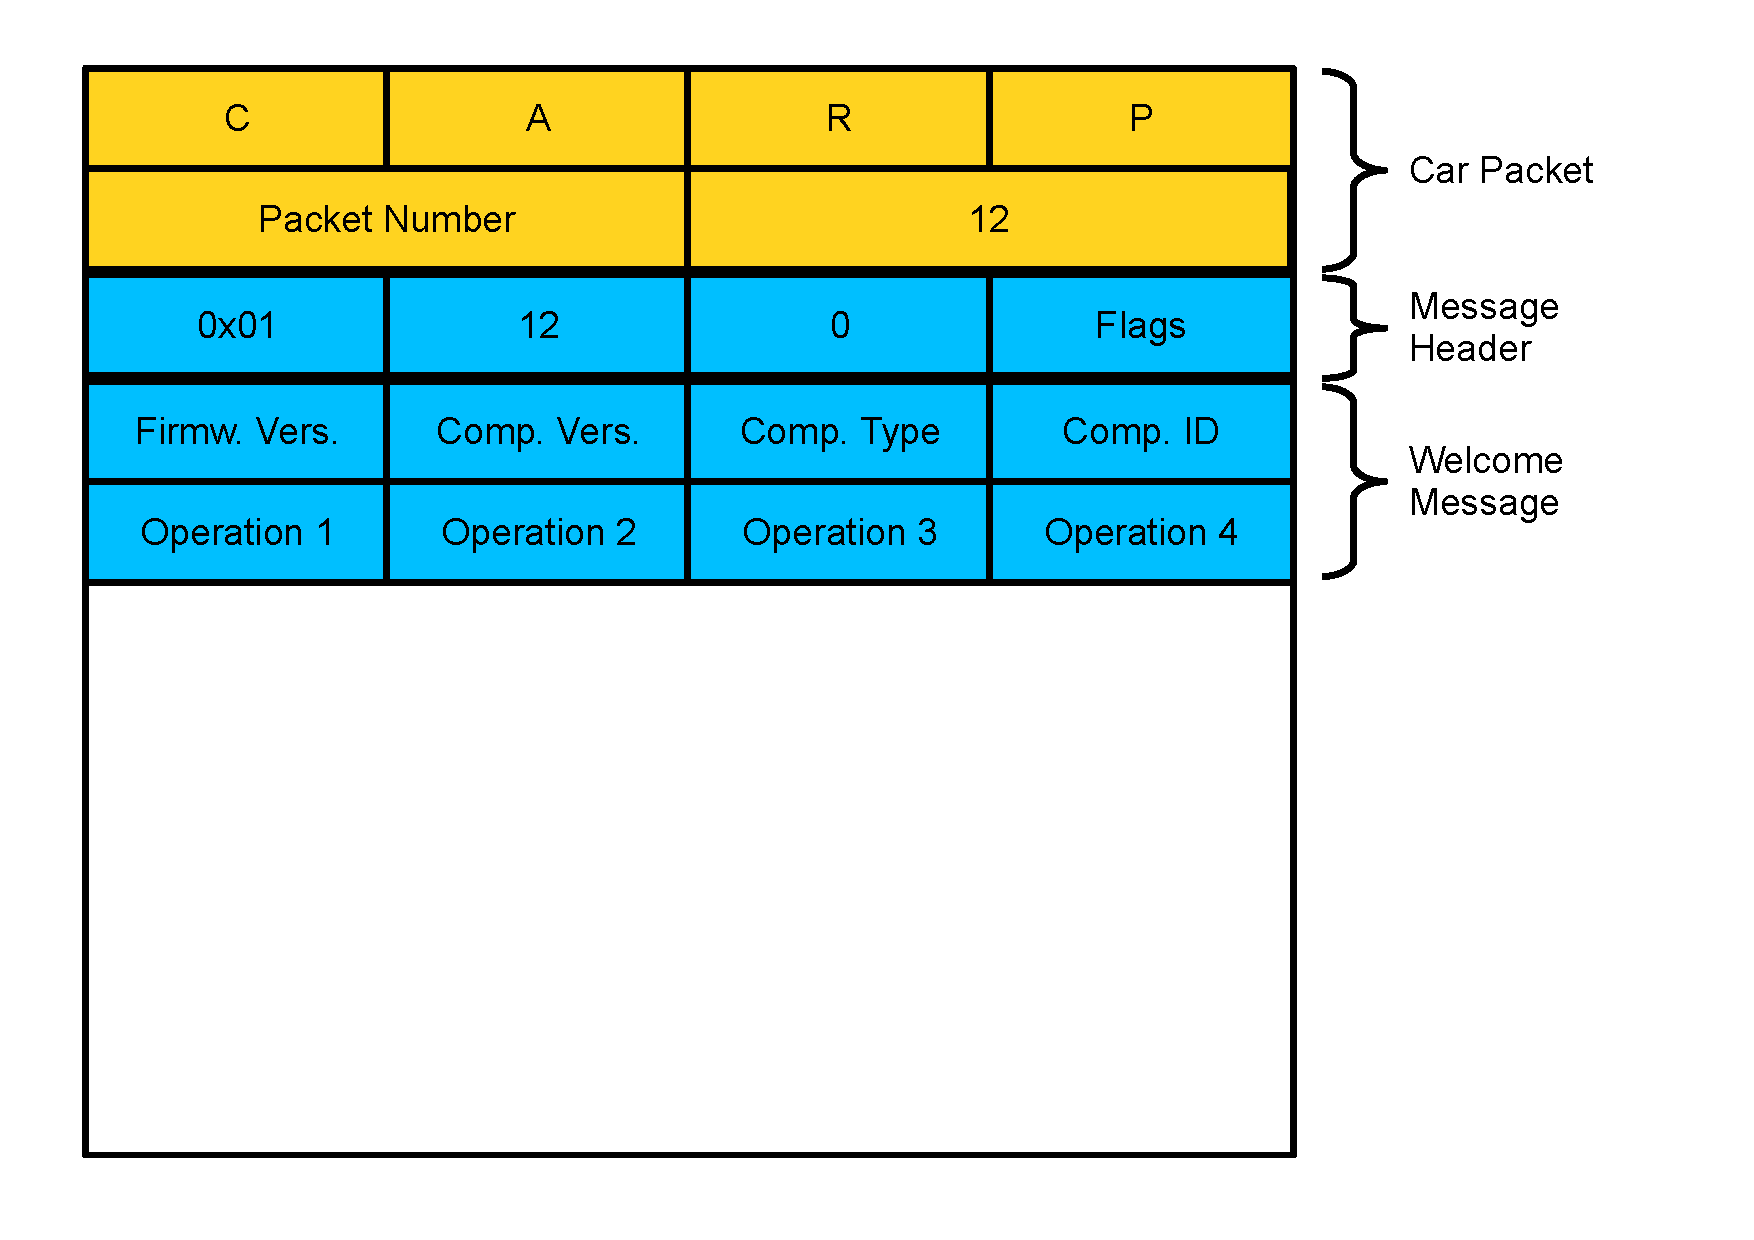
\includegraphics[scale=0.35]{figures/prot2.pdf}
\end{frame}

\begin{frame}
	\frametitle{Networking Protocol}
	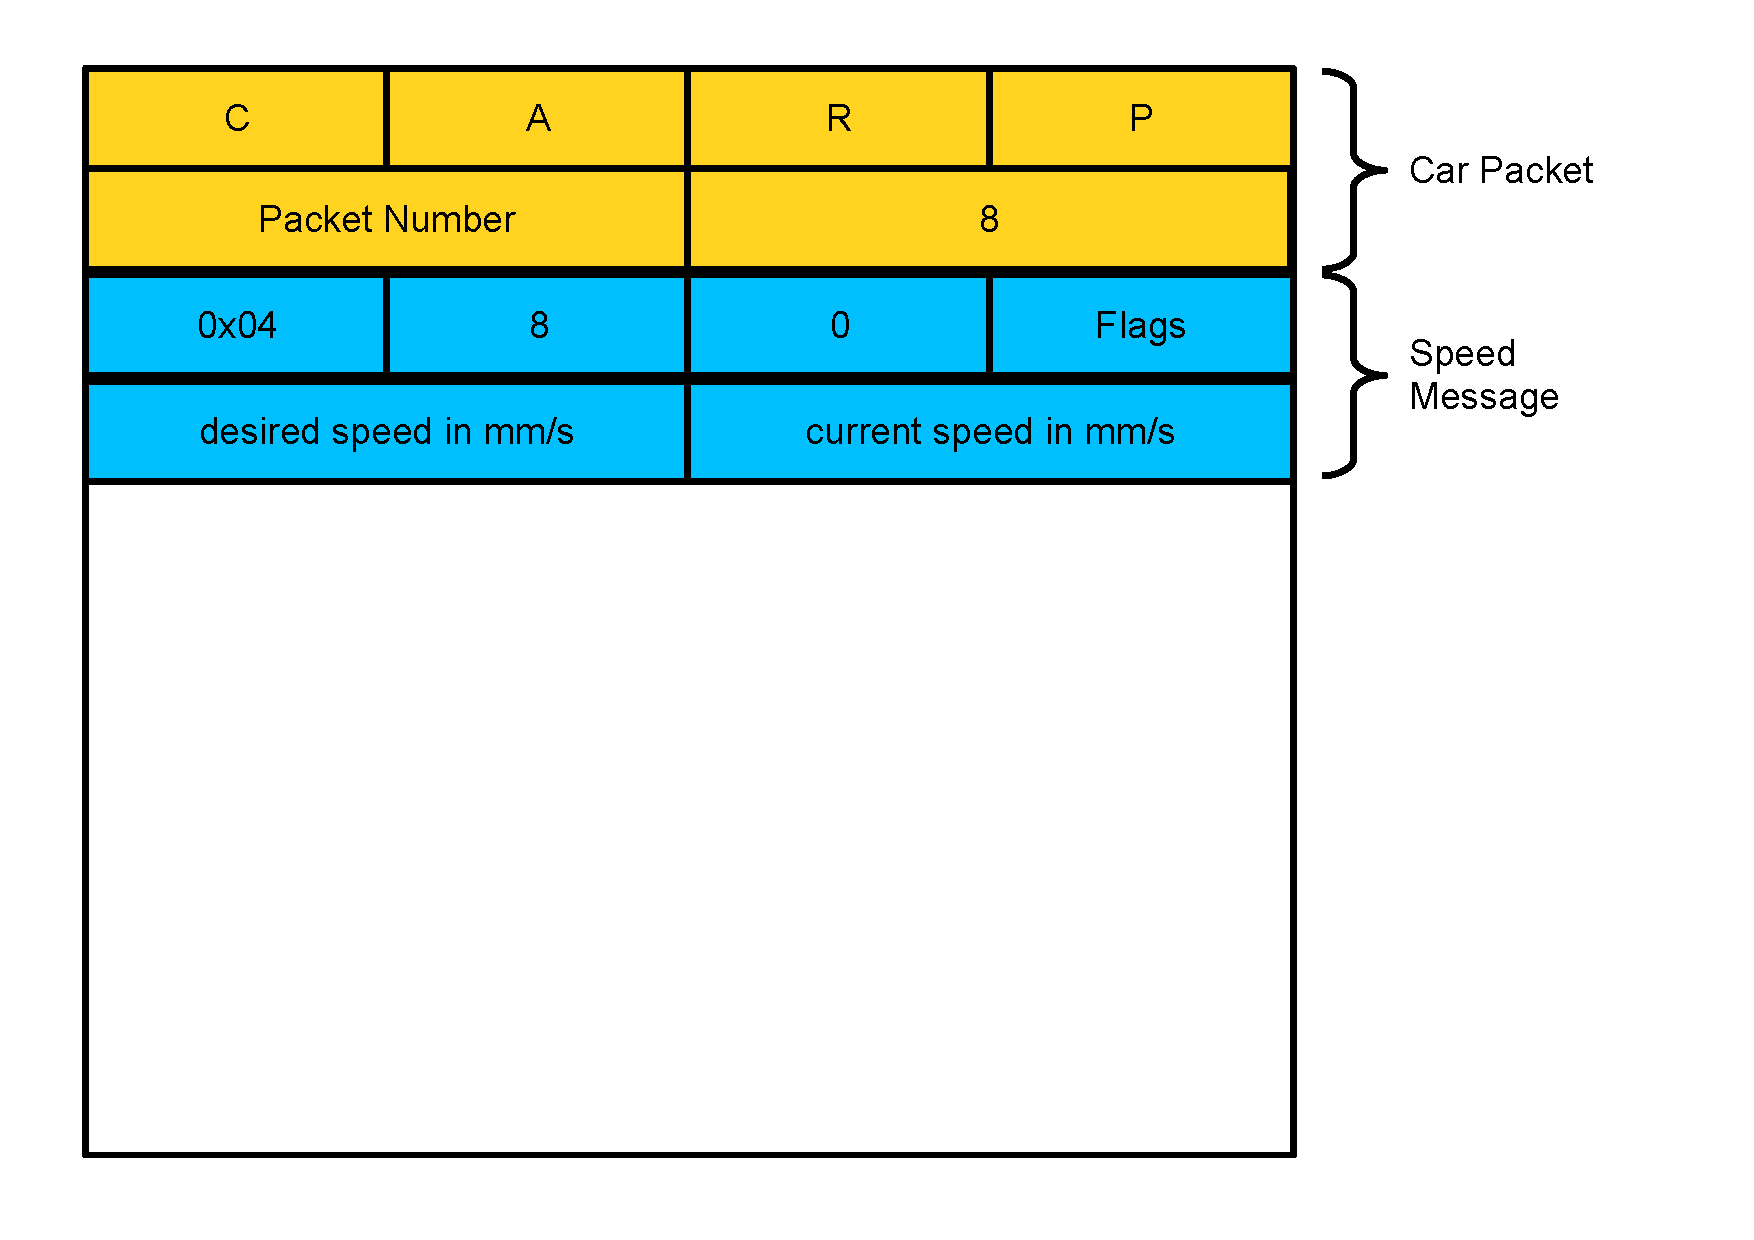
\includegraphics[scale=0.35]{figures/prot3.pdf}
\end{frame}

\begin{frame}
	\frametitle{Networking Protocol}
	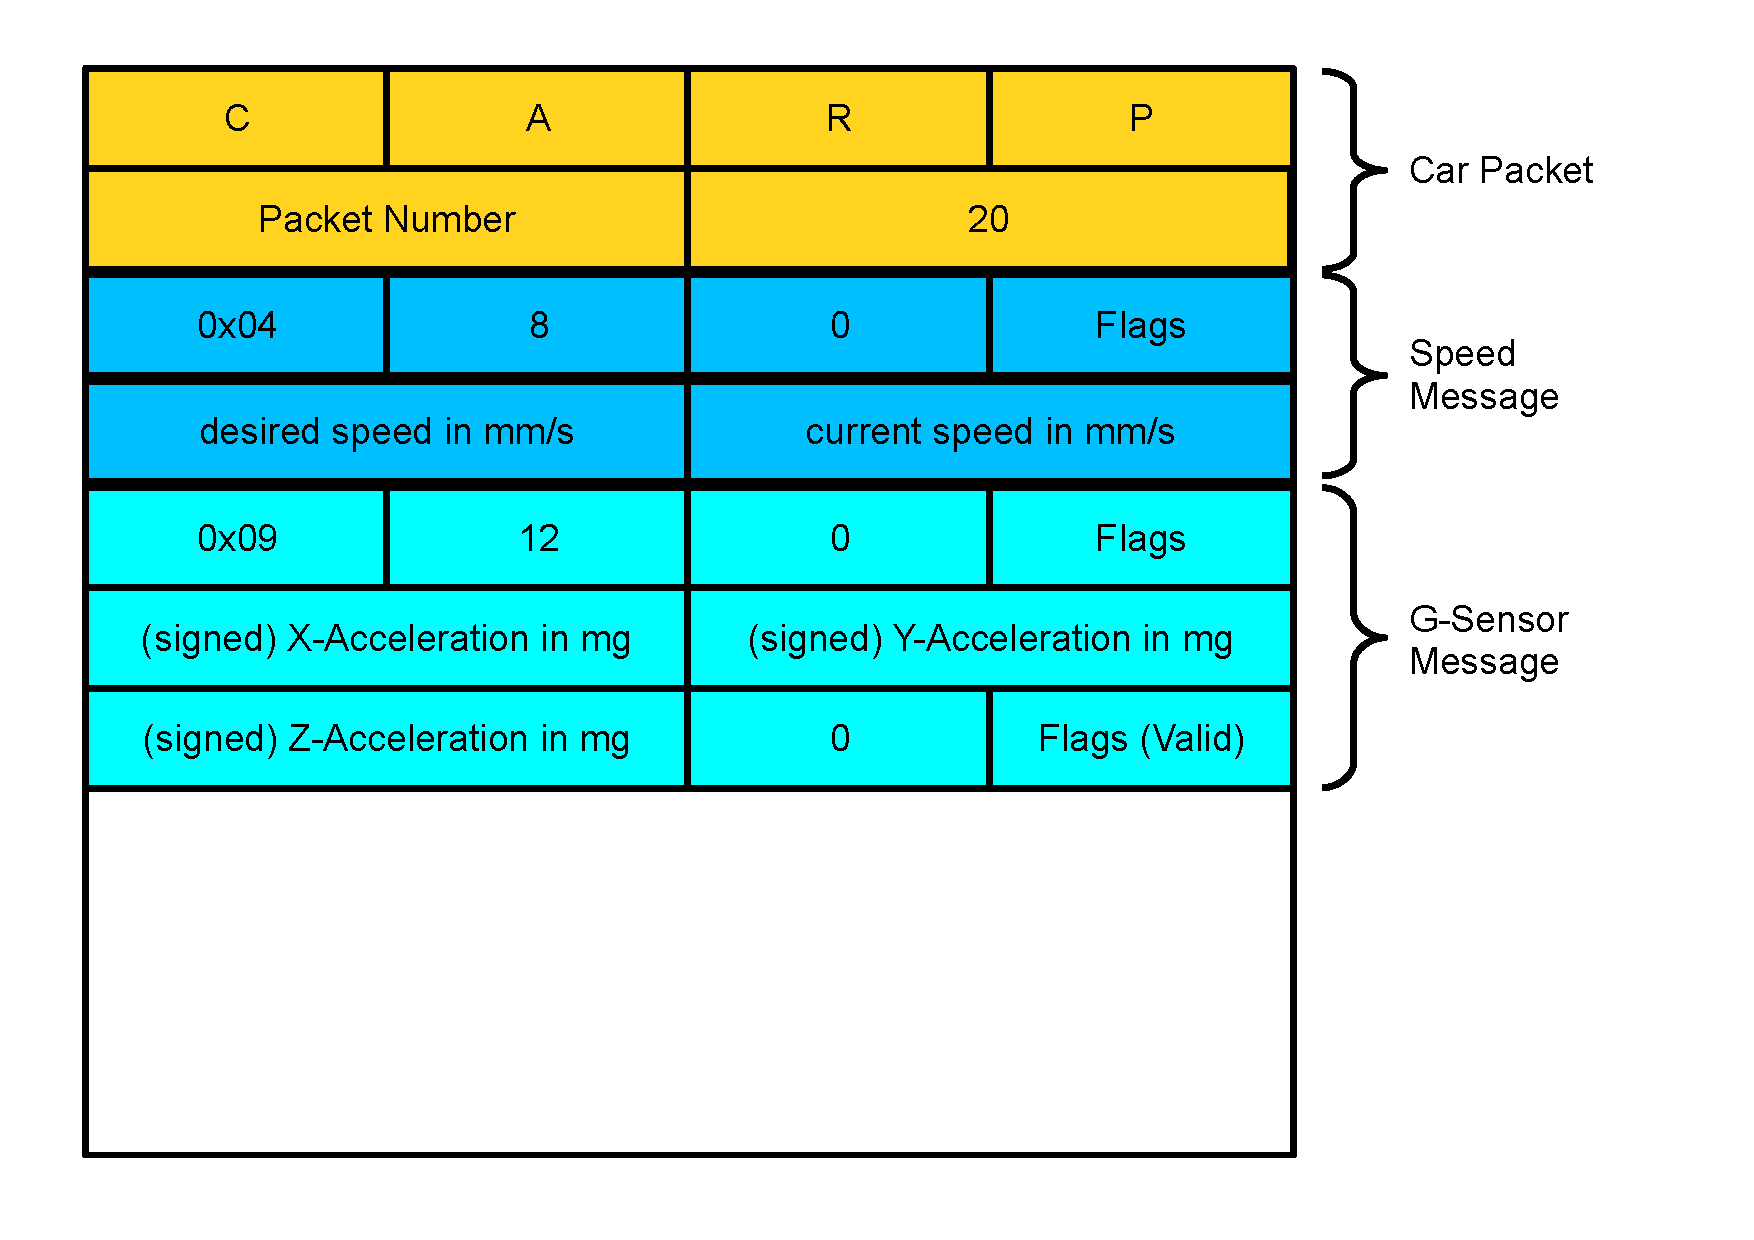
\includegraphics[scale=0.35]{figures/prot4.pdf}
\end{frame}


\begin{frame}
	\frametitle{Network Architecture}
	\begin{itemize}
		\item single star-architecture
		\item components communicate only with the central Linux-PC, not each other
		\item components only understand the protocols they need
		\item[] exception: CarPacket (main protocol) and messages with type lower 8
		\item similar components can use different protocols\\
		(e.g. CMW-Units from different producers)
	\end{itemize}
\end{frame}

\begin{frame}
	\frametitle{Network Architecture}
	\includegraphics[scale=0.7]{figures/connection.jpg}
\end{frame}



\section{Central ECU Architecture}

\subsection{Linux-PC}

\begin{frame}
	\frametitle{Central ECU: Linux-PC}
	Processing Unit: \textsl{Sabre-light i.mx6} development board (4 cores).\\ \vspace{1em}	
	
	Main tasks:
	\begin{enumerate}
		\item Control the speed-controller
		\item (Polling the sensors)
		\item Calculate next behavior
	\end{enumerate}
\end{frame}

\begin{frame}
	\frametitle{Central ECU: Linux-PC}
	SW Architecture:
	\begin{itemize}
		\item Multi-Process / Multi-Thread
		\item seperated Behavior-Planning and Network-Communication
	\end{itemize} \vspace{1em}
	
	Current Setup:
	\begin{itemize}
		\item Main application: 
		\begin{itemize}
			\item 1. Thread: network-communication
			\item 2. Thread: web-communication
			\item Main Thread: behavior-planning
		\end{itemize}		 
		\item Web-Server for control-ui
		\item dhcp-server, os, much more ;)
	\end{itemize}
\end{frame}

\begin{frame}
	\frametitle{Central ECU: Linux-PC}
	Current Behavior:
	\begin{itemize}
		\item Human user controls movements via GUI
		\item GUI sends data to a hidden server (not NSA)
		\item If car is in danger (see wall ;)) then the car will speed down.
		\item If the distance between car and obstacle is lower 20 cm then the car will stop.
	\end{itemize}
\end{frame}

\begin{frame}
	\frametitle{Central ECU: Linux-PC}
	Possible Behavior:
	\begin{itemize}
		\item Car discovers the world around it
		\item ABS, ESP via G-Sensors (data is already available)
		\item Web-Cam for little NSA-agents ;)
		\item ...
	\end{itemize}
\end{frame}

\section*{}

\begin{frame}
	\frametitle{Thank You!}
	\center{ {\huge Thank you for your attention!}}
	
	\center{{\huge  Any (even silly) questions???}}
\end{frame}

\end{document}
